\documentclass[../../main.tex]{subfiles}
\begin{document}

\begin{flushright}
\footnotesize\textit{【自動文字起こし・要確認】}
\end{flushright}

{\bf [解]}
$C_1:y=\sqrt3\log(x+1)$，$C_2:y=\sqrt3\log(1-x)$である．

円$C$の半径を$r\ (>0)$とすると，$\triangle ABP$が正三角形であるから，$A$，$B$の$x$座標は順に$\dfrac12r$，$-\dfrac12r$である．さらに$P(0,a)$とおくと，$A$での$C_1$の接線$\ell_1$は
\begin{align*}
\ell_1:y=\frac{\sqrt3}{1+\frac12r}\left(x-\frac12r\right)+\sqrt3\log\left(1+\frac12r\right)
\end{align*}
であり，半径$PA\perp\ell_1$かつ$PA$と$y$軸のなす角が$30^\circ$であることから，$\ell_1$の傾きが$\tan30^\circ=\dfrac{\sqrt3}3$だから，
\begin{align*}
\frac{\sqrt3}{1+\frac12r}=\frac{\sqrt3}{3}\quad\therefore\ r=4\quad\cdots①
\end{align*}

この時，$a$を$2$通りで表して
\begin{align*}
a=\sqrt3\log\left(1+\frac12r\right)+\frac{\sqrt3}2r=\sqrt3\log3+2\sqrt3\quad\cdots②
\end{align*}
である．

\begin{figure}[htb]
\centering
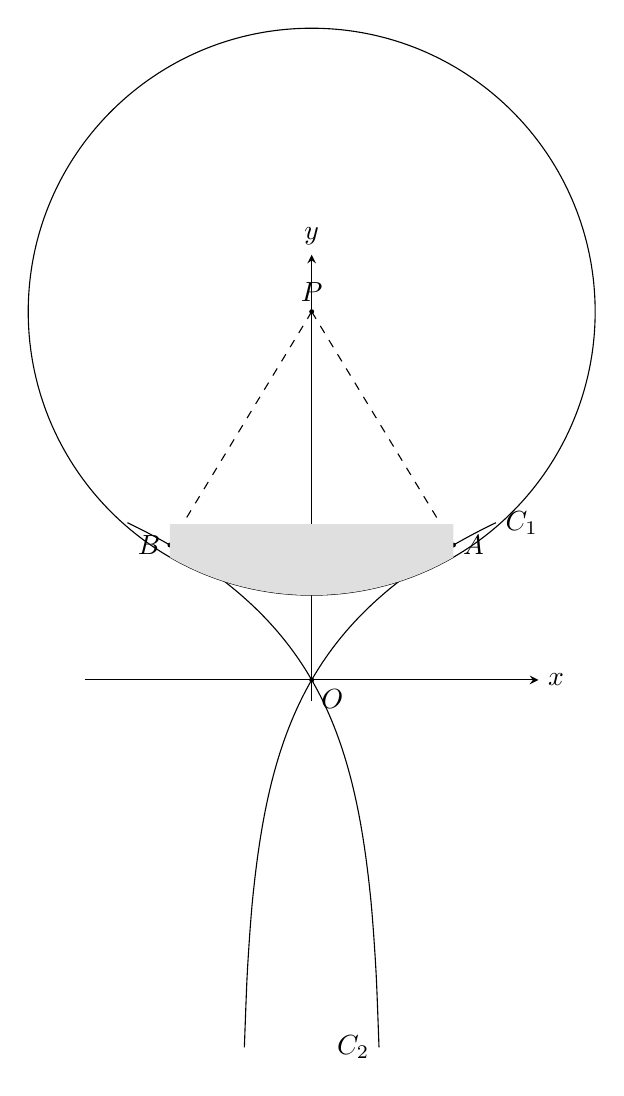
\begin{tikzpicture}[scale=0.9, >=stealth]
  \draw[->] (-3.2,0) -- (3.2,0) node[right] {$x$};
  \draw[->] (0,-0.3) -- (0,6) node[above] {$y$};
  \draw[domain=-0.95:2.6, samples=100, smooth] plot (\x, {sqrt(3)*ln(\x+1)}) node[right] {$C_1$};
  \draw[domain=-2.6:0.95, samples=100, smooth] plot (\x, {sqrt(3)*ln(1-\x)}) node[left] {$C_2$};
  \draw (0,5.196) circle (4);
  \fill (0,5.196) circle (1pt) node[above] {$P$};
  \fill (2,1.903) circle (1pt) node[right] {$A$};
  \fill (-2,1.903) circle (1pt) node[left] {$B$};
  \fill (0,0) circle (1pt) node[below right] {$O$};
  \draw[dashed] (0,5.196) -- (2,1.903);
  \draw[dashed] (0,5.196) -- (-2,1.903);
  \begin{scope}
    \clip (-2,0) rectangle (2,2.2);
    \clip (0,5.196) circle (4);
    \fill[gray!25] (-2.2,-0.2) rectangle (2.2,2.2);
  \end{scope}
\end{tikzpicture}
\caption{円$C$と曲線$C_1$，$C_2$で囲まれた部分（斜線部）}
\end{figure}

求める面積を$S$とする．対称性から
\begin{align*}
\frac12S=(\text{台形}OAP)-(\text{$C_1$と$x$軸，$x=2$で囲まれた部分})-(\text{中心$P$，半径$r$，中心角$\pi/6$の扇形})\quad\cdots③
\end{align*}
であり，
\begin{align*}
\text{台形}OAP&=\frac12\{\sqrt3\log3+a\}\cdot2=\sqrt3\log3+a，\\
\int_0^2\sqrt3\log(x+1)\,dx&=\sqrt3\Bigl[(x+1)\log(x+1)-(x+1)\Bigr]_0^2=\sqrt3(3\log3-2)，\\
\text{扇形}&=\frac12\cdot\frac\pi6\cdot r^2=\frac43\pi
\end{align*}

を②とあわせて③から
\begin{align*}
\frac12S&=2\sqrt3\log3+2\sqrt3-\left(3\sqrt3\log3-2\sqrt3+\frac43\pi\right)\\
&=4\sqrt3-\sqrt3\log3-\frac43\pi
\end{align*}
\begin{align*}
\therefore\ S=2\left(4\sqrt3-\sqrt3\log3-\frac43\pi\right)．
\end{align*}

\newpage

\end{document}
